\documentclass{beamer}
\usepackage[english,activeacute]{babel}
\usepackage[utf8]{inputenc}
\usepackage{listings}
\usepackage{algorithmic}
\usepackage{color}

\definecolor{gray2}{rgb}{100,100,100}
\definecolor{red}{rgb}{255,0,0}
\definecolor{blue}{rgb}{0,0,255}
\definecolor{gray97}{gray}{.97}
\definecolor{gray75}{gray}{.75}
\definecolor{gray45}{gray}{.45}

\newcommand{\blue}{\textcolor{blue}}
\newcommand{\red}{\textcolor{red}}
\newcommand{\green}{\textcolor{green}}


\usetheme[pageofpages=of,% String used between the current page and the
                         % total page count.
          alternativetitlepage=true,% Use the fancy title page.
          titlepagelogo=img/logo,% Logo for the first page.
          watermark=,% Watermark used in every page.
          watermarkheight=100px,% Height of the watermark.
          watermarkheightmult=4,% The watermark image is 4 times bigger
                                % than watermarkheight.
          ]{Torino}

\usecolortheme{nouvelle}

\author[C. Maureira]{\large Cristián Maureira Fredes\\\normalsize \textcolor{gray}{cmaureir@csrg.cl}}
\title[Solving Strip-Packing using Scatter-Search]{Solving the strip-packing problem, using a scatter-search meta-heuristic}
\institute[UTFSM]{Departamento de Informática\\Universidad Técnica Federico Santa María}
\date{\today}

\begin{document}
\begin{frame}[t,plain]
\titlepage
\end{frame}
\frame
{
\frametitle{N-body problem}
\begin{block}{Definition}
    Predict the \underline{movement} of a \underline{celestial objects} group,
    which are \underline{interacting} with each other \underline{gravitationally}.
\end{block}
}

\frame
{
\frametitle{N-body problem}
\begin{itemize}
    \item Dynamic simulation of a particle system.
    \item Applications.
    \begin{itemize}
        \item Fluid mechanics
        \item Astrophysics
        \item Stellar dynamics
        \item Video games
        \item etc.
    \end{itemize}
\end{itemize}
}


\frame
{
\frametitle{N-body problem}
Critical sections:
\begin{itemize}
    \item Initial positions.
    \item Integration method.
    \item Force calculation.
\end{itemize}
}


\frame
{
\frametitle{N-body problem}

\begin{itemize}
    \item Force calculation.
    \begin{itemize}
        \item Initial positions $x_i$.
        \item Initial velocities $v_i$.
        \item $1 \leq i \leq N$
    \end{itemize}
    $$f_{ij} =G \cdot \frac{m_i \cdot m_j}{||r_{ij}||^{2}} \cdot \frac{r_{ij}}{||r_ij||}$$
    \begin{itemize}
        \item $m_i$ and $m_j$ masses of the $i$ and $j$ bodies.
        \item $r_{ij} = (x_j - x_i )$ distance vector between the $i$ and $j$ bodies.
        \item $G$, gravitational constant. ($6,67428 \times 10^{-11} m^{3} kg^{-1} s^{-2}$)
    \end{itemize}
\end{itemize}
}

Given a set of N rectangles of with width ($w_{i}$) and height ($h_{i}$),
the 2D strip-packing problem aims to pack each rectangle on a strip
with a defined width ($W$), and an infinite height ($H$).

The main goal is to minimize the height on the strip
generated by the placement of all the rectangle,
minimizing also the free space between the rectangles.

The position of each rectangle on the strip is defined
by the coordinates of the bottom-left corner $(a_{i},b_{i})$.

This model can be formulated as follows:

\begin{eqnarray}
\text{Minimize H}\nonumber \\
\text{Subject to}\nonumber \\
a_{i} + w_{i} \leq W, \forall i \in N \\
b_{i} + h_{i} \leq H, \forall i \in N \\
a_{i} + w_{i} \leq a_{j}\text{ or }a_{j} + w_{j} \leq a_{i}\text{ or }\nonumber\\
b_{i} + h_{i} \leq b_{j}\text{ or }b_{j} + h_{j} \leq b_{i}, \forall (i,j) \in N, i\neq j\\
a_{i} + b_{i} \geq 0. \forall i \in N.
\end{eqnarray}

In this case,
the scenerio of the proposed algorithm is a non-guillotinable
and based on bottom-left heuristic, which does consider as invalid
the rectangle overlapping.

\begin{frame}[fragile]
    \frametitle{Methodology}
    \framesubtitle{Algorithm}

    \begin{algorithm}[H]
        \scriptsize
        \begin{algorithmic}
            \STATE solution\_generation()
            \STATE solution\_improvement()
            \STATE refset\_build()
            \STATE save\_the\_best\_solution()
            \REPEAT
                \WHILE {$\text{New solutions in RefSet}$}
                    \STATE solution\_combination()
                    \STATE solution\_improvement()
                    \STATE refSet\_modification()
                \ENDWHILE
                \STATE save\_the\_best\_solution()
                \STATE refset\_rebuild()
            \UNTIL {iteration $<$ Max\_Iteration}
        \end{algorithmic}
        \caption{Scatter Search Procedure}
        \label{alg:1}
    \end{algorithm}

\end{frame}


\begin{frame}
    \frametitle{Methodology}
    \framesubtitle{Solution improvement}

        \begin{figure}[h!t]
            \centering
            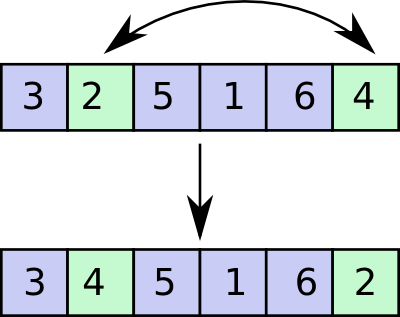
\includegraphics[width=0.3\textwidth]{../report/img/ia-swap}
            \caption{Swap movement to improve solutions example. $N/2$ times.}
            \label{fig:swap}
        \end{figure}

\end{frame}

\begin{frame}
    \frametitle{Methodology}
    \framesubtitle{Solution combination}

        \begin{figure}[h!t]
            \centering
            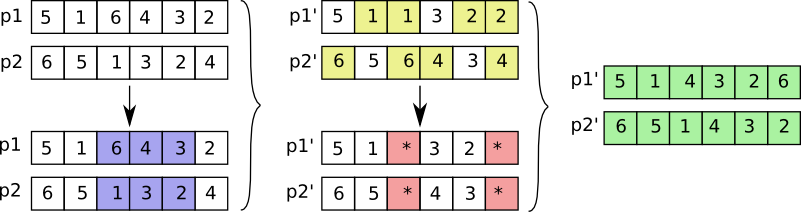
\includegraphics[width=0.8\textwidth]{../report/img/ia-pmx}
            \caption{Partial Matching Crossover (PMX) example.}
            \label{fig:pmx}
        \end{figure}

\end{frame}


\begin{frame}
    \frametitle{Methodology}
    \framesubtitle{RefSet rebuild}

        \begin{figure}[h!t]
            \centering
            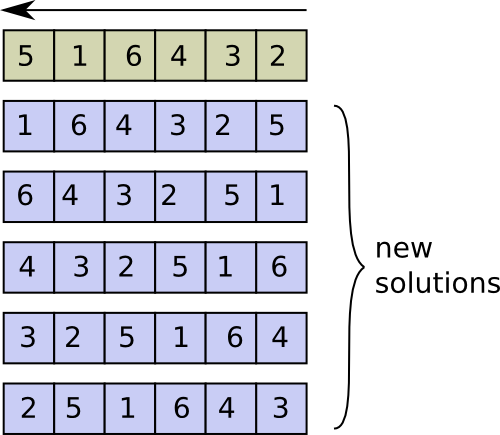
\includegraphics[width=0.5\textwidth]{../report/img/ia-shift}
            \caption{Shift example.}
            \label{fig:shift}
        \end{figure}

\end{frame}

\begin{frame}
    \frametitle{Computational tests}
    \framesubtitle{Hardware}

    \begin{table}
        \centering
        \begin{tabular}{|l|r|}
            \hline
            \textbf{Processor} & Phenom II X4 965 Black AM3 3.4Ghz\\\hline
            \textbf{RAM} & 8GB 1333MHz\\\hline
            \textbf{OS} & Arch Linux, Kernel 3.2.11 \\\hline
        \end{tabular}
        \label{tab:table1}
        \caption{Hardware configuration}
    \end{table}

\end{frame}

\begin{frame}
    \frametitle{Computational tests}
    \framesubtitle{Parameters}

    \begin{itemize}
        \item Selection parameter ($b = 10$)
        \item Solutions number    ($popsize = b*5$)
        \item Maximum iteration   ($max\_iter = 100$)
    \end{itemize}

\end{frame}

\begin{frame}
    \frametitle{Computational tests}
    \framesubtitle{Results (1/2)}

    \begin{table}[H]
        \centering
        \small
        \begin{tabular}{|c|c|c|c|c|}
            \hline
            \textbf{Instance} & \textbf{Elements} & \textbf{Time (*)} & \textbf{Height} & \textbf{Height (**)} \\ \hline
            c1-p1 (HT01)      & 17                & 0.103s        & 20              & 20                  \\ \hline
            c1-p2 (HT02)      & 18                & 2.823s        & 21              & 20                  \\ \hline
            c1-p3 (HT03)      & 17                & 0.427s        & 20              & 20                  \\ \hline
            c2-p1 (HT04)      & 26                & 7.463s        & 16              & 15                  \\ \hline
            c2-p2 (HT05)      & 26                & 5.870s        & 16              & 15                  \\ \hline
            c2-p3 (HT06)      & 26                & 6.263s        & 16              & 15                  \\ \hline
            c3-p1 (HT07)      & 29                & 22.006s       & 32              & 30                  \\ \hline
            c3-p2 (HT08)      & 30                & 20.812s       & 32              & 30                  \\ \hline
            c3-p3 (HT09)      & 29                & 20.952s       & 32              & 30                  \\ \hline
        \end{tabular}
        \label{tab:results}
        \caption{Best solutions using Hopper and Turton benchmark input 
    data. (*) User + Sys time, using \texttt{time} unix command. (**) means the optimal height.}
    \end{table}
\end{frame}

\begin{frame}
    \frametitle{Computational tests}
    \framesubtitle{Results (2/2)}

    \begin{table}[H]
        \centering
        \small
        \begin{tabular}{|c|c|c|c|c|}
            \hline
            \textbf{Instance} & \textbf{Elements} & \textbf{Time (*)} & \textbf{Height} & \textbf{Height (**)} \\ \hline
            c4-p1             & 49                & 2m 7.795s     & 64              & 60                  \\ \hline
            c4-p2             & 49                & 2m 18.007s    & 64              & 60                  \\ \hline
            c4-p3             & 49                & 1m 52.080s    & 63              & 60                  \\ \hline
            c5-p1             & 73                & 5m 50.928s    & 94              & 90                  \\ \hline
            c5-p2             & 73                & 5m 48.117s    & 96              & 90                  \\ \hline
            c5-p3             & 73                & 5m 17.333s    & 94              & 90                  \\ \hline
            c6-p1             & 98                & 13m 53.045s   & 127             & 120                 \\ \hline
            c6-p2             & 98                & 13m 36.017s   & 127             & 120                 \\ \hline
            c6-p3             & 98                & 13m 34.047s   & 127             & 120                 \\ \hline
            c7-p1             & 196               & 151m 15.409s  & X             & 240                 \\ \hline
            c7-p2             & 197               & 206m 4.504s   & X             & 240                 \\ \hline
            c7-p3             & 196               & 236m 47.587s  & X             & 240                 \\ \hline
        \end{tabular}
        \label{tab:results}
        \caption{Best solutions using Hopper and Turton benchmark input 
    data. (*) User + Sys time, using \texttt{time} unix command. (**) means the optimal height.}
    \end{table}
\end{frame}


\begin{frame}
    \frametitle{Computational tests}
    \framesubtitle{Diagram (HT01)}

    \begin{center}
      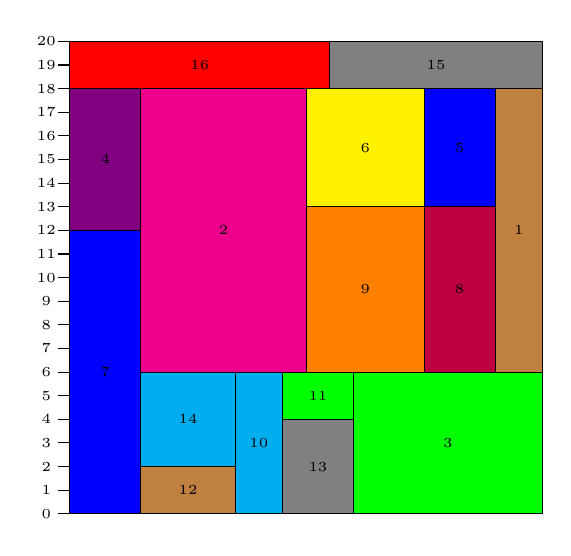
\begin{tikzpicture}[scale=0.3]
        \tikzstyle{every node}=[font=\tiny]
        \begin{scope}
       \foreach\x in {0,1,2,...,20}{
            \node at (-1,\x) {\x};
            \draw (-0.5,\x) -- (0,\x);
        }
           \draw (0 ,20) -- (0,0) -- (20,0) -- (20,20);
               \filldraw[blue,draw=black] (0,0) rectangle (3,12);
               \draw (1.5,6) node {7};

               \filldraw[brown,draw=black] (3,0) rectangle (7,2);
               \draw (5,1) node {12};

               \filldraw[cyan,draw=black] (7,0) rectangle (9,6);
               \draw (8,3) node {10};

               \filldraw[gray,draw=black] (9,0) rectangle (12,4);
               \draw (10.5,2) node {13};

               \filldraw[green,draw=black] (12,0) rectangle (20,6);
               \draw (16,3) node {3};

               \filldraw[magenta,draw=black] (3,6) rectangle (10,18);
               \draw (6.5,12) node {2};

               \filldraw[orange,draw=black] (10,6) rectangle (15,13);
               \draw (12.5,9.5) node {9};

               \filldraw[purple,draw=black] (15,6) rectangle (18,13);
               \draw (16.5,9.5) node {8};

               \filldraw[red,draw=black] (0,18) rectangle (11,20);
               \draw (5.5,19) node {16};

               \filldraw[violet,draw=black] (0,12) rectangle (3,18);
               \draw (1.5,15) node {4};

               \filldraw[yellow,draw=black] (10,13) rectangle (15,18);
               \draw (12.5,15.5) node {6};

               \filldraw[blue,draw=black] (15,13) rectangle (18,18);
               \draw (16.5,15.5) node {5};

               \filldraw[brown,draw=black] (18,6) rectangle (20,18);
               \draw (19,12) node {1};

               \filldraw[cyan,draw=black] (3,2) rectangle (7,6);
               \draw (5,4) node {14};

               \filldraw[gray,draw=black] (11,18) rectangle (20,20);
               \draw (15.5,19) node {15};

               \filldraw[green,draw=black] (9,4) rectangle (12,6);
               \draw (10.5,5) node {11};

         \end{scope}
      \end{tikzpicture}
    \end{center}
\end{frame}

\begin{frame}
    \frametitle{Computational tests}
    \framesubtitle{Diagram (HT03)}

    \begin{center}

  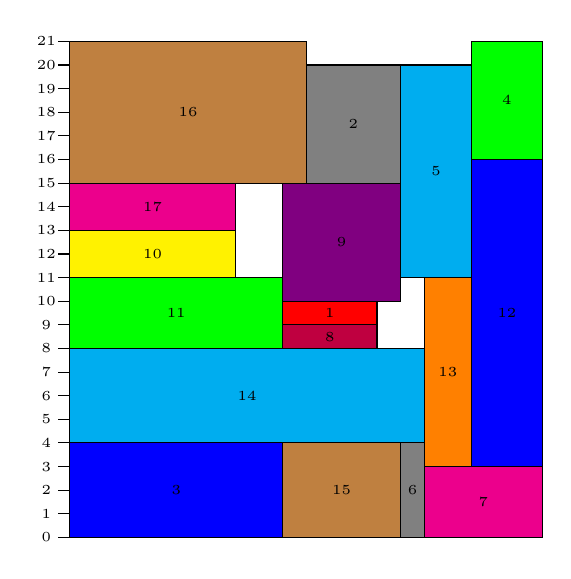
\begin{tikzpicture}[scale=0.3]
    \tikzstyle{every node}=[font=\tiny]
    \begin{scope}

       \foreach\x in {0,1,2,...,21}{
            \node at (-1,\x) {\x};
            \draw (-0.5,\x) -- (0,\x);
        }
       \draw (0 ,21) -- (0,0) -- (20,0) -- (20,21);
           \filldraw[blue,draw=black] (0,0) rectangle (9,4);
           \draw (4.5,2) node {3};

           \filldraw[brown,draw=black] (9,0) rectangle (14,4);
           \draw (11.5,2) node {15};

           \filldraw[cyan,draw=black] (0,4) rectangle (15,8);
           \draw (7.5,6) node {14};

           \filldraw[gray,draw=black] (14,0) rectangle (15,4);
           \draw (14.5,2) node {6};

           \filldraw[green,draw=black] (0,8) rectangle (9,11);
           \draw (4.5,9.5) node {11};

           \filldraw[magenta,draw=black] (15,0) rectangle (20,3);
           \draw (17.5,1.5) node {7};

           \filldraw[orange,draw=black] (15,3) rectangle (17,11);
           \draw (16,7) node {13};

           \filldraw[purple,draw=black] (9,8) rectangle (13,9);
           \draw (11,8.5) node {8};

           \filldraw[red,draw=black] (9,9) rectangle (13,10);
           \draw (11,9.5) node {1};

           \filldraw[violet,draw=black] (9,10) rectangle (14,15);
           \draw (11.5,12.5) node {9};

           \filldraw[yellow,draw=black] (0,11) rectangle (7,13);
           \draw (3.5,12) node {10};

           \filldraw[blue,draw=black] (17,3) rectangle (20,16);
           \draw (18.5,9.5) node {12};

           \filldraw[brown,draw=black] (0,15) rectangle (10,21);
           \draw (5,18) node {16};

           \filldraw[cyan,draw=black] (14,11) rectangle (17,20);
           \draw (15.5,15.5) node {5};

           \filldraw[gray,draw=black] (10,15) rectangle (14,20);
           \draw (12,17.5) node {2};

           \filldraw[green,draw=black] (17,16) rectangle (20,21);
           \draw (18.5,18.5) node {4};

           \filldraw[magenta,draw=black] (0,13) rectangle (7,15);
           \draw (3.5,14) node {17};

     \end{scope}
  \end{tikzpicture}

    \end{center}
\end{frame}

\begin{frame}
    \frametitle{Computational tests}
    \framesubtitle{Diagram (c4-p1)}

    \begin{center}


      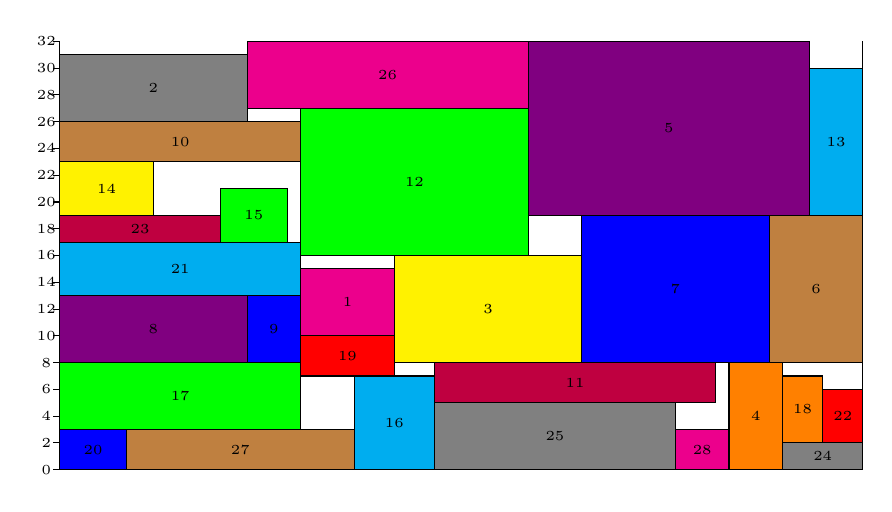
\begin{tikzpicture}[scale=0.17]
        \tikzstyle{every node}=[font=\tiny]
        \begin{scope}
       \foreach\x in {0,2,...,32}{
            \node at (-1,\x) {\x};
            \draw (-0.5,\x) -- (0,\x);
        }
       \draw (0 ,32) -- (0,0) -- (60,0) -- (60,32);
           \filldraw[blue,draw=black] (0,0) rectangle (5,3);
           \draw (2.5,1.5) node {20};

           \filldraw[brown,draw=black] (5,0) rectangle (22,3);
           \draw (13.5,1.5) node {27};

           \filldraw[cyan,draw=black] (22,0) rectangle (28,7);
           \draw (25,3.5) node {16};

           \filldraw[gray,draw=black] (28,0) rectangle (46,5);
           \draw (37,2.5) node {25};

           \filldraw[green,draw=black] (0,3) rectangle (18,8);
           \draw (9,5.5) node {17};

           \filldraw[magenta,draw=black] (46,0) rectangle (50,3);
           \draw (48,1.5) node {28};

           \filldraw[orange,draw=black] (50,0) rectangle (54,8);
           \draw (52,4) node {4};

           \filldraw[purple,draw=black] (28,5) rectangle (49,8);
           \draw (38.5,6.5) node {11};

           \filldraw[red,draw=black] (18,7) rectangle (25,10);
           \draw (21.5,8.5) node {19};

           \filldraw[violet,draw=black] (0,8) rectangle (14,13);
           \draw (7,10.5) node {8};

           \filldraw[yellow,draw=black] (25,8) rectangle (39,16);
           \draw (32,12) node {3};

           \filldraw[blue,draw=black] (39,8) rectangle (53,19);
           \draw (46,13.5) node {7};

           \filldraw[brown,draw=black] (53,8) rectangle (60,19);
           \draw (56.5,13.5) node {6};

           \filldraw[cyan,draw=black] (0,13) rectangle (18,17);
           \draw (9,15) node {21};

           \filldraw[gray,draw=black] (54,0) rectangle (60,2);
           \draw (57,1) node {24};

           \filldraw[green,draw=black] (18,16) rectangle (35,27);
           \draw (26.5,21.5) node {12};

           \filldraw[magenta,draw=black] (18,10) rectangle (25,15);
           \draw (21.5,12.5) node {1};

           \filldraw[orange,draw=black] (54,2) rectangle (57,7);
           \draw (55.5,4.5) node {18};

           \filldraw[purple,draw=black] (0,17) rectangle (12,19);
           \draw (6,18) node {23};

           \filldraw[red,draw=black] (57,2) rectangle (60,6);
           \draw (58.5,4) node {22};

           \filldraw[violet,draw=black] (35,19) rectangle (56,32);
           \draw (45.5,25.5) node {5};

           \filldraw[yellow,draw=black] (0,19) rectangle (7,23);
           \draw (3.5,21) node {14};

           \filldraw[blue,draw=black] (14,8) rectangle (18,13);
           \draw (16,10.5) node {9};

           \filldraw[brown,draw=black] (0,23) rectangle (18,26);
           \draw (9,24.5) node {10};

           \filldraw[cyan,draw=black] (56,19) rectangle (60,30);
           \draw (58,24.5) node {13};

           \filldraw[gray,draw=black] (0,26) rectangle (14,31);
           \draw (7,28.5) node {2};

           \filldraw[green,draw=black] (12,17) rectangle (17,21);
           \draw (14.5,19) node {15};

           \filldraw[magenta,draw=black] (14,27) rectangle (35,32);
           \draw (24.5,29.5) node {26};

     \end{scope}
  \end{tikzpicture}


    \end{center}
\end{frame}

\begin{frame}
    \frametitle{Computational tests}
    \framesubtitle{Diagram (c5-p1)}

    \begin{center}

      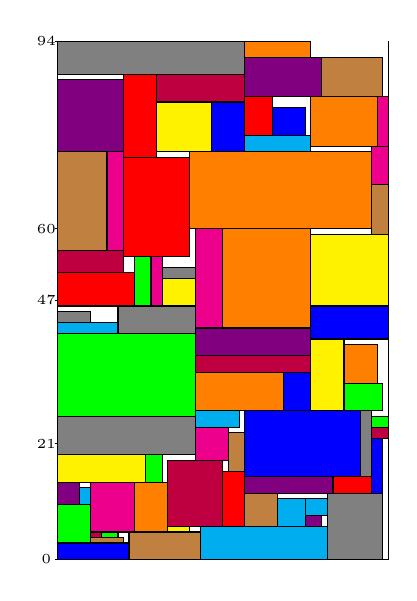
\begin{tikzpicture}[scale=0.07]
        \tikzstyle{every node}=[font=\tiny]
        \begin{scope}
       \foreach\x in {0,21,47,60,94}{
            \node at (-2,\x) {\x};
            \draw (-0.5,\x) -- (0,\x);
        }

       \draw (0 ,94) -- (0,0) -- (60,0) -- (60,94);
           \filldraw[blue,draw=black] (0,0) rectangle (13,3);

           \filldraw[brown,draw=black] (13,0) rectangle (26,5);

           \filldraw[cyan,draw=black] (26,0) rectangle (49,6);

           \filldraw[gray,draw=black] (49,0) rectangle (59,12);

           \filldraw[green,draw=black] (0,3) rectangle (6,10);

           \filldraw[magenta,draw=black] (6,5) rectangle (14,14);

           \filldraw[orange,draw=black] (14,5) rectangle (20,14);

           \filldraw[purple,draw=black] (20,6) rectangle (30,18);

           \filldraw[red,draw=black] (30,6) rectangle (34,16);

           \filldraw[violet,draw=black] (34,12) rectangle (50,15);

           \filldraw[yellow,draw=black] (0,14) rectangle (16,19);

           \filldraw[blue,draw=black] (34,15) rectangle (55,27);

           \filldraw[brown,draw=black] (34,6) rectangle (40,12);

           \filldraw[cyan,draw=black] (40,6) rectangle (45,11);

           \filldraw[gray,draw=black] (0,19) rectangle (25,26);

           \filldraw[green,draw=black] (0,26) rectangle (25,41);

           \filldraw[magenta,draw=black] (25,18) rectangle (31,24);

           \filldraw[orange,draw=black] (25,27) rectangle (41,34);

           \filldraw[purple,draw=black] (25,34) rectangle (46,37);

           \filldraw[red,draw=black] (50,12) rectangle (57,15);

           \filldraw[violet,draw=black] (25,37) rectangle (46,42);

           \filldraw[yellow,draw=black] (46,27) rectangle (52,40);

           \filldraw[blue,draw=black] (46,40) rectangle (60,46);

           \filldraw[brown,draw=black] (6,3) rectangle (12,4);

           \filldraw[cyan,draw=black] (0,41) rectangle (11,43);

           \filldraw[gray,draw=black] (11,41) rectangle (25,46);

           \filldraw[green,draw=black] (52,27) rectangle (59,32);

           \filldraw[magenta,draw=black] (25,42) rectangle (30,60);

           \filldraw[orange,draw=black] (30,42) rectangle (46,60);

           \filldraw[purple,draw=black] (6,4) rectangle (8,5);

           \filldraw[red,draw=black] (0,46) rectangle (14,52);

           \filldraw[violet,draw=black] (45,6) rectangle (48,8);

           \filldraw[yellow,draw=black] (46,46) rectangle (60,59);

           \filldraw[blue,draw=black] (57,12) rectangle (59,22);

           \filldraw[brown,draw=black] (31,16) rectangle (34,23);

           \filldraw[cyan,draw=black] (45,8) rectangle (49,11);

           \filldraw[gray,draw=black] (55,15) rectangle (57,27);

           \filldraw[green,draw=black] (14,46) rectangle (17,55);

           \filldraw[magenta,draw=black] (17,46) rectangle (19,55);

           \filldraw[orange,draw=black] (52,32) rectangle (58,39);

           \filldraw[purple,draw=black] (0,52) rectangle (12,56);

           \filldraw[red,draw=black] (12,55) rectangle (24,73);

           \filldraw[violet,draw=black] (0,10) rectangle (4,14);

           \filldraw[yellow,draw=black] (19,46) rectangle (25,51);

           \filldraw[blue,draw=black] (41,27) rectangle (46,34);

           \filldraw[brown,draw=black] (0,56) rectangle (9,74);

           \filldraw[cyan,draw=black] (25,24) rectangle (33,27);

           \filldraw[gray,draw=black] (0,43) rectangle (6,45);

           \filldraw[green,draw=black] (16,14) rectangle (19,19);

           \filldraw[magenta,draw=black] (9,56) rectangle (12,74);

           \filldraw[orange,draw=black] (24,60) rectangle (57,74);

           \filldraw[purple,draw=black] (57,22) rectangle (60,24);

           \filldraw[red,draw=black] (12,73) rectangle (18,88);

           \filldraw[violet,draw=black] (0,74) rectangle (12,87);

           \filldraw[yellow,draw=black] (18,74) rectangle (28,83);

           \filldraw[blue,draw=black] (28,74) rectangle (34,83);

           \filldraw[brown,draw=black] (57,59) rectangle (60,68);

           \filldraw[cyan,draw=black] (34,74) rectangle (46,77);

           \filldraw[gray,draw=black] (19,51) rectangle (25,53);

           \filldraw[green,draw=black] (8,4) rectangle (11,5);

           \filldraw[magenta,draw=black] (57,68) rectangle (60,75);

           \filldraw[orange,draw=black] (46,75) rectangle (58,84);

           \filldraw[purple,draw=black] (18,83) rectangle (34,88);

           \filldraw[red,draw=black] (34,77) rectangle (39,84);

           \filldraw[violet,draw=black] (34,84) rectangle (48,91);

           \filldraw[yellow,draw=black] (20,5) rectangle (24,6);

           \filldraw[blue,draw=black] (39,77) rectangle (45,82);

           \filldraw[brown,draw=black] (48,84) rectangle (59,91);

           \filldraw[cyan,draw=black] (4,10) rectangle (6,13);

           \filldraw[gray,draw=black] (0,88) rectangle (34,94);

           \filldraw[green,draw=black] (57,24) rectangle (60,26);

           \filldraw[magenta,draw=black] (58,75) rectangle (60,84);

           \filldraw[orange,draw=black] (34,91) rectangle (46,94);

     \end{scope}
  \end{tikzpicture}



    \end{center}
\end{frame}

\begin{frame}
    \frametitle{Computational tests}
    \framesubtitle{Diagram (c6-p1)}

    \begin{center}


      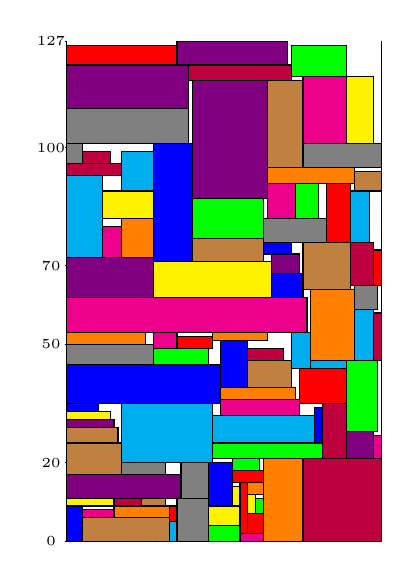
\begin{tikzpicture}[scale=0.05]
        \tikzstyle{every node}=[font=\tiny]
        \begin{scope}
       \foreach\x in {0,20,50,70,100,127}{
            \node at (-4,\x) {\x};
            \draw (-0.5,\x) -- (0,\x);
        }
       \draw (0 ,127) -- (0,0) -- (80,0) -- (80,127);
           \filldraw[blue,draw=black] (0,0) rectangle (4,9);

           \filldraw[brown,draw=black] (4,0) rectangle (26,6);

           \filldraw[cyan,draw=black] (26,0) rectangle (28,5);

           \filldraw[gray,draw=black] (28,0) rectangle (36,11);

           \filldraw[green,draw=black] (36,0) rectangle (44,4);

           \filldraw[magenta,draw=black] (44,0) rectangle (50,2);

           \filldraw[orange,draw=black] (50,0) rectangle (60,21);

           \filldraw[purple,draw=black] (60,0) rectangle (80,21);

           \filldraw[red,draw=black] (44,2) rectangle (46,15);

           \filldraw[violet,draw=black] (0,11) rectangle (29,17);

           \filldraw[yellow,draw=black] (36,4) rectangle (44,9);

           \filldraw[blue,draw=black] (36,9) rectangle (42,20);

           \filldraw[brown,draw=black] (0,17) rectangle (14,25);

           \filldraw[cyan,draw=black] (14,20) rectangle (37,35);

           \filldraw[gray,draw=black] (29,11) rectangle (36,20);

           \filldraw[green,draw=black] (37,21) rectangle (65,25);

           \filldraw[magenta,draw=black] (4,6) rectangle (12,8);

           \filldraw[orange,draw=black] (12,6) rectangle (26,9);

           \filldraw[purple,draw=black] (65,21) rectangle (71,35);

           \filldraw[red,draw=black] (46,2) rectangle (50,7);

           \filldraw[violet,draw=black] (71,21) rectangle (78,28);

           \filldraw[yellow,draw=black] (0,9) rectangle (12,11);

           \filldraw[blue,draw=black] (0,35) rectangle (39,45);

           \filldraw[brown,draw=black] (0,25) rectangle (13,29);

           \filldraw[cyan,draw=black] (37,25) rectangle (63,32);

           \filldraw[gray,draw=black] (14,17) rectangle (25,20);

           \filldraw[green,draw=black] (71,28) rectangle (79,46);

           \filldraw[magenta,draw=black] (39,32) rectangle (59,36);

           \filldraw[orange,draw=black] (39,36) rectangle (58,39);

           \filldraw[purple,draw=black] (12,9) rectangle (19,11);

           \filldraw[red,draw=black] (59,35) rectangle (71,44);

           \filldraw[violet,draw=black] (0,29) rectangle (12,31);

           \filldraw[yellow,draw=black] (0,31) rectangle (11,33);

           \filldraw[blue,draw=black] (39,39) rectangle (46,51);

           \filldraw[brown,draw=black] (46,39) rectangle (57,46);

           \filldraw[cyan,draw=black] (57,44) rectangle (62,53);

           \filldraw[gray,draw=black] (0,45) rectangle (22,50);

           \filldraw[green,draw=black] (22,45) rectangle (36,49);

           \filldraw[magenta,draw=black] (0,53) rectangle (61,62);

           \filldraw[orange,draw=black] (62,46) rectangle (73,64);

           \filldraw[purple,draw=black] (46,46) rectangle (55,49);

           \filldraw[red,draw=black] (42,15) rectangle (50,18);

           \filldraw[violet,draw=black] (0,62) rectangle (22,72);

           \filldraw[yellow,draw=black] (22,62) rectangle (52,71);

           \filldraw[blue,draw=black] (52,62) rectangle (60,68);

           \filldraw[brown,draw=black] (60,64) rectangle (72,76);

           \filldraw[cyan,draw=black] (73,46) rectangle (78,59);

           \filldraw[gray,draw=black] (73,59) rectangle (79,65);

           \filldraw[green,draw=black] (42,18) rectangle (49,21);

           \filldraw[magenta,draw=black] (22,49) rectangle (28,53);

           \filldraw[orange,draw=black] (0,50) rectangle (20,53);

           \filldraw[purple,draw=black] (72,65) rectangle (78,76);

           \filldraw[red,draw=black] (26,5) rectangle (28,9);

           \filldraw[violet,draw=black] (52,68) rectangle (59,73);

           \filldraw[yellow,draw=black] (46,7) rectangle (48,12);

           \filldraw[blue,draw=black] (22,71) rectangle (32,101);

           \filldraw[brown,draw=black] (32,71) rectangle (50,77);

           \filldraw[cyan,draw=black] (0,72) rectangle (9,93);

           \filldraw[gray,draw=black] (50,76) rectangle (66,82);

           \filldraw[green,draw=black] (32,77) rectangle (50,87);

           \filldraw[magenta,draw=black] (9,72) rectangle (14,80);

           \filldraw[orange,draw=black] (14,72) rectangle (22,82);

           \filldraw[purple,draw=black] (78,46) rectangle (80,58);

           \filldraw[red,draw=black] (66,76) rectangle (72,91);

           \filldraw[violet,draw=black] (32,87) rectangle (51,117);

           \filldraw[yellow,draw=black] (9,82) rectangle (22,89);

           \filldraw[blue,draw=black] (63,25) rectangle (65,34);

           \filldraw[brown,draw=black] (19,9) rectangle (25,11);

           \filldraw[cyan,draw=black] (72,76) rectangle (77,89);

           \filldraw[gray,draw=black] (0,101) rectangle (31,110);

           \filldraw[green,draw=black] (48,7) rectangle (50,11);

           \filldraw[magenta,draw=black] (51,82) rectangle (58,91);

           \filldraw[orange,draw=black] (51,91) rectangle (73,95);

           \filldraw[purple,draw=black] (0,93) rectangle (14,96);

           \filldraw[red,draw=black] (28,49) rectangle (37,52);

           \filldraw[violet,draw=black] (0,110) rectangle (31,121);

           \filldraw[yellow,draw=black] (42,9) rectangle (44,14);

           \filldraw[blue,draw=black] (0,33) rectangle (8,35);

           \filldraw[brown,draw=black] (51,95) rectangle (60,117);

           \filldraw[cyan,draw=black] (14,89) rectangle (22,99);

           \filldraw[gray,draw=black] (60,95) rectangle (80,101);

           \filldraw[green,draw=black] (58,82) rectangle (64,91);

           \filldraw[magenta,draw=black] (60,101) rectangle (71,118);

           \filldraw[orange,draw=black] (37,51) rectangle (51,53);

           \filldraw[purple,draw=black] (31,117) rectangle (57,121);

           \filldraw[red,draw=black] (0,121) rectangle (28,126);

           \filldraw[violet,draw=black] (28,121) rectangle (56,127);

           \filldraw[yellow,draw=black] (71,101) rectangle (78,118);

           \filldraw[blue,draw=black] (50,73) rectangle (57,76);

           \filldraw[brown,draw=black] (73,89) rectangle (80,94);

           \filldraw[cyan,draw=black] (62,44) rectangle (71,46);

           \filldraw[gray,draw=black] (0,96) rectangle (4,101);

           \filldraw[green,draw=black] (57,118) rectangle (71,126);

           \filldraw[magenta,draw=black] (78,21) rectangle (80,27);

           \filldraw[orange,draw=black] (46,12) rectangle (50,15);

           \filldraw[purple,draw=black] (4,96) rectangle (11,99);

           \filldraw[red,draw=black] (78,65) rectangle (80,74);

     \end{scope}
  \end{tikzpicture}

    \end{center}
\end{frame}

\begin{frame}
    \frametitle{Computational tests}
    \framesubtitle{Diagram (c7-p1)}

    \begin{center}


    \end{center}
\end{frame}

\begin{frame}
    \frametitle{Conclusion and future work}
    \framesubtitle{}
    \begin{itemize}
        \item Execution time vs Solution quality.
        \item Stagnation (solution improvement).
        \item Rotation.
    \end{itemize}
\end{frame}

\begin{frame}[t,plain]
\titlepage
\end{frame}
\end{document}
